\documentclass[14pt,a4paper]{extarticle}
\usepackage[T2A]{fontenc}
\usepackage[utf8]{inputenc}
\usepackage[english,russian]{babel}
\usepackage{lmodern}
\usepackage{geometry}
\usepackage{array}
\usepackage{tabularx}
\usepackage{longtable}
\usepackage{ltablex}
\usepackage{booktabs}
\usepackage[hidelinks]{hyperref}
\usepackage{indentfirst}
\usepackage[protrusion=true,expansion=false]{microtype}
\usepackage{graphicx}
\usepackage{setspace}
\usepackage{listings}
\usepackage[justification=centering]{caption}
\usepackage{float}
\usepackage{tocloft}
\usepackage{titlesec}
\usepackage{newtxtext,newtxmath}

\titleformat{\section}
  {\normalfont\bfseries}
  {\thesection.}
  {2mm}
  {}
\titlespacing*{\section}{1.5cm}{*3}{*1}

\titleformat{\subsection}
  {\normalfont\bfseries}
  {\thesubsection.}
  {2mm}
  {}
\titlespacing*{\subsection}{1.5cm}{*3}{*1}

\captionsetup[figure]{labelsep=endash, name={Рисунок}}
\captionsetup[table]{labelsep=endash, name={Таблица}}
\renewcommand{\thefigure}{\arabic{figure}}
\renewcommand{\thetable}{\arabic{table}}
\makeatletter
\def\fnum@table{\tablename~\thetable}
\def\fnum@figure{\figurename~\thefigure}
\long\def\@makecaption#1#2{%
  \vskip\abovecaptionskip
  \centering
  #1~---~#2\par
  \vskip\belowcaptionskip}
\makeatother
\setlength{\abovecaptionskip}{6pt}
\setlength{\belowcaptionskip}{8pt}
\keepXColumns
\setlength{\parindent}{3em}
\newgeometry{left=2.5cm,right=2.5cm,top=3cm,bottom=2.5cm}
\setlength{\tabcolsep}{4pt}
\setlength{\emergencystretch}{2em}
\graphicspath{{./}{pdf/}{../results/}{results/}}

\renewcommand{\contentsname}{\hspace*{4em}{\small Содержание}}
\setlength{\cftbeforesecskip}{0.5em}
\renewcommand{\cftsecleader}{\cftdotfill{\cftdotsep}}
\renewcommand{\cftsecaftersnum}{.\hspace{2mm}}

\lstset{language=Python, basicstyle=\ttfamily\small, breaklines=true,
        frame=single, columns=fullflexible, keepspaces=true}

\title{Отчёт по лабораторной работе №3 «Классификация, поиск и RAG: анализ узких мест»}
\author{Выполнил студент группы М-РИТ-25-1, Станиславчук С.М.}

\begin{document}

\setstretch{1.5}
\noindent
\begin{minipage}[c]{0.15\textwidth}
    
\includegraphics[width=\linewidth]{LSTU.jpg}
\end{minipage}\hfill
\begin{minipage}[c]{0.82\textwidth}
    \centering
    {\small
    МИНИСТЕРСТВО НАУКИ И ВЫСШЕГО ОБРАЗОВАНИЯ РФ \\[1em]
    ФЕДЕРАЛЬНОЕ ГОСУДАРСТВЕННОЕ БЮДЖЕТНОЕ \\
    ОБРАЗОВАТЕЛЬНОЕ УЧРЕЖДЕНИЕ ВЫСШЕГО ОБРАЗОВАНИЯ \\
    «ЛИПЕЦКИЙ ГОСУДАРСТВЕННЫЙ ТЕХНИЧЕСКИЙ УНИВЕРСИТЕТ»
    }
\end{minipage}%

\vspace{3em}

\noindent
\hspace{1em}%
\begin{minipage}[t]{0.8\textwidth}
\textbf{Институт} \hspace{2em} компьютерных наук \\
\textbf{Кафедра} \hspace{2em} автоматизированных систем управления
\end{minipage}

\vspace{6em}

\begin{center}
\textbf{Лабораторная работа №3} \\
по дисциплине \\
<<Прикладные задачи искусственного интеллекта>>
\end{center}

\vspace{6em}

\noindent
\begin{tabular*}{\textwidth}{@{\extracolsep{\fill}} l c r }
    Студент М-РИТ-25-1 & \makebox[4cm]{\hrulefill} & Станиславчук С.М. \\[2em]
Руководитель & \\
Профессор & \makebox[4cm]{\hrulefill} & Седых И.А. \\
\end{tabular*}

\vfill
\begin{center}
    Липецк, 2026
\end{center}

\thispagestyle{empty}

\newpage
\tableofcontents
\newpage

\section{Задание}

\textbf{Вариант 16.} Спортивные форумы 20 Newsgroups (подмножество \texttt{rec.*}).
Датасет --- \texttt{SetFit/\allowbreak 20\_newsgroups}; классы части~1:
\texttt{rec.\allowbreak autos}, \texttt{rec.\allowbreak motorcycles},
\texttt{rec.sport.\allowbreak baseball}, \texttt{rec.sport.\allowbreak hockey}. Вопросы без ответа для части~3 --- травмы игроков,
не попавшие в сообщения. Номер варианта $VARIANT=16$, зерно
$SEED=42$ (фиксируется для \texttt{random}, \texttt{numpy} и \texttt{torch}).

Цель работы --- настроить три ключевых компонента RAG-системы (классификатор,
поисковый индекс и генератор) и найти узкие места архитектуры по качеству выдачи.
Работа состоит из трёх частей с весами 20\,\%, 30\,\% и 50\,\%:
\begin{enumerate}
    \item классификация документов без обучения и с дообучением
          \texttt{cointegrated/\allowbreak rubert-tiny2};
    \item плотный поиск по базе знаний при трёх размерах чанка (S, M, L);
    \item RAG с гибридным поиском (BM25 + dense, RRF) и генератором
          \texttt{Qwen/Qwen2.5-0.5B-Instruct}, сравнение трёх промптов.
\end{enumerate}

Пул данных после фильтрации и перемешивания содержит 3874 документа;
разбиение Train/Test --- 3099/775 (80/20). Для частей~2 и~3 база знаний ---
300 документов тестовой части. Стек: Python, Hugging Face Transformers и Datasets,
Sentence Transformers, FAISS, \texttt{rank\_bm25}, Matplotlib. Версии библиотек:
torch 2.15, transformers 5.12, datasets 5.0.1, sentence-transformers 6.2,
faiss-cpu 1.15.1, rank\_bm25 0.2.2.

\section{Ход работы}

\subsection{Часть 1. Классификация: без обучения и с дообучением}

\textbf{Эксперимент A (без обучения).} Модель \texttt{cointegrated/rubert-tiny2}
с \texttt{max\_seq\_length=256} кодирует тестовые документы и четыре описания
классов (\texttt{cars}, \texttt{motorcycles}, \texttt{baseball}, \texttt{hockey}).
Класс документа --- описание с максимальной косинусной близостью к эмбеддингу
документа.

\textbf{Эксперимент B (дообучение).} Та же модель с линейной головой над
\texttt{[CLS]}: 5 эпох, скорость обучения $2\cdot10^{-5}$, батч 32,
\texttt{max\_length=256}, валидация после каждой эпохи, \texttt{SEED=42}.

\begin{lstlisting}
# Experiment A: zero-shot classification
st = SentenceTransformer("cointegrated/rubert-tiny2")
st.max_seq_length = 256
E_doc = st.encode(test_ds["text"], normalize_embeddings=True, batch_size=64)
E_cls = st.encode(CLASS_TEXTS, normalize_embeddings=True)
pred_a = (E_doc @ E_cls.T).argmax(1)

# Experiment B: linear head over [CLS]
model = AutoModelForSequenceClassification.from_pretrained(
    "cointegrated/rubert-tiny2", num_labels=len(CLASSES))
args = TrainingArguments(num_train_epochs=5, learning_rate=2e-5,
                         per_device_train_batch_size=32,
                         eval_strategy="epoch", seed=SEED)
trainer = Trainer(model=model, args=args, train_dataset=enc(train_ds),
                  eval_dataset=enc(test_ds), data_collator=collator)
trainer.train()
pred_b = trainer.predict(enc(test_ds)).predictions.argmax(-1)
\end{lstlisting}
\refstepcounter{figure}
\captionof*{figure}{Классификация: эксперименты A (косинус) и B (дообучение)}
\label{fig:clf-code}

Результаты на тестовой выборке приведены в таблице~\ref{tab:clf}.

\begin{table}[H]
    \centering
    \refstepcounter{table}
    \caption*{\raggedleft Accuracy и F1-macro на тестовой выборке (775 документов)}
    \label{tab:clf}
    \begin{tabular}{lrrr}
        \toprule
        Метод & Accuracy & F1-macro & Время, с \\
        \midrule
        A: косинус с описаниями классов & 0.3381 & 0.2858 & 44.7 \\
        B: дообучение ruBERT-tiny2     & 0.7535 & 0.7510 & 5261.6 \\
        \bottomrule
    \end{tabular}
\end{table}

Дообучение дало прирост \textbf{Accuracy $+0.4155$} (0.3381 $\to$ 0.7535) и
\textbf{F1-macro $+0.4652$} (0.2858 $\to$ 0.7510). Обучение заняло 5261.6~с
(около 88~мин) на CPU; инференс без обучения --- 44.7~с. Нулевой baseline
с косинусом работает лишь немного лучше случайного выбора из четырёх классов
(0.25), что подтверждает необходимость специализации модели под предметную область.

Матрица ошибок эксперимента~B приведена на рисунке~\ref{fig:cm}.

\begin{figure}[H]
    \centering
    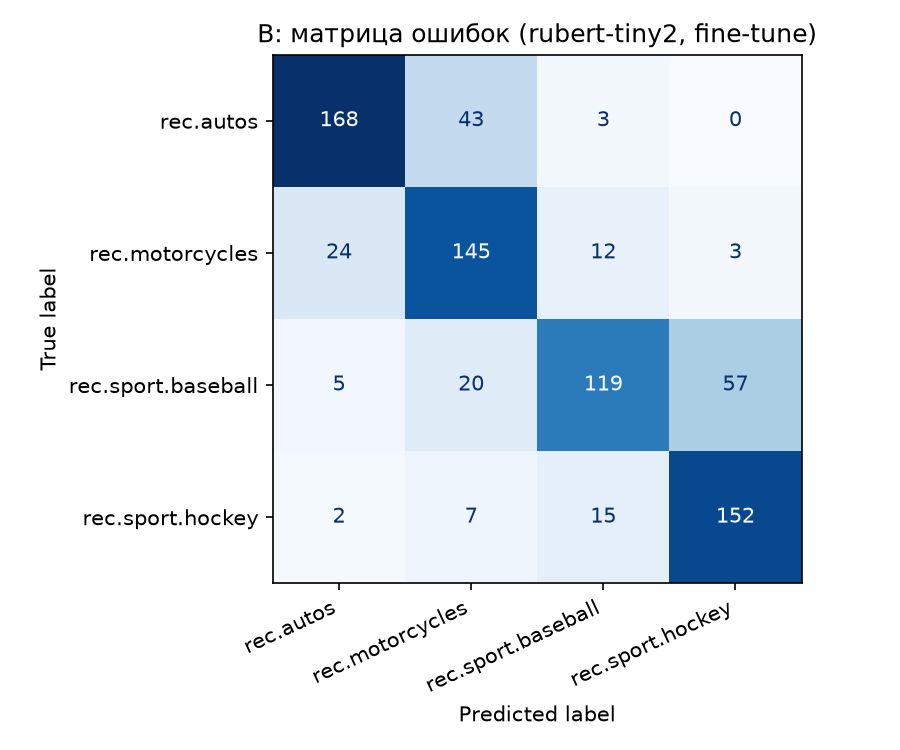
\includegraphics[width=0.64\textwidth]{confusion_matrix.png}
    \refstepcounter{figure}
    \caption*{Матрица ошибок ruBERT-tiny2 после дообучения (B)}
    \label{fig:cm}
\end{figure}

Самые частые пары ошибок собраны в таблице~\ref{tab:confused}.

\begin{table}[H]
    \centering
    \refstepcounter{table}
    \caption*{\raggedleft Наиболее частые ошибки классификатора}
    \label{tab:confused}
    \begin{tabular}{llr}
        \toprule
        Истинный класс & Предсказанный класс & Ошибок \\
        \midrule
        \texttt{rec.sport.baseball} & \texttt{rec.sport.hockey}      & 57 \\
        \texttt{rec.autos}          & \texttt{rec.motorcycles}       & 43 \\
        \texttt{rec.motorcycles}    & \texttt{rec.autos}             & 24 \\
        \texttt{rec.sport.baseball} & \texttt{rec.motorcycles}       & 20 \\
        \bottomrule
    \end{tabular}
\end{table}

Самая частая пара --- \texttt{rec.sport.baseball} $\to$ \texttt{rec.sport.hockey}
(57 ошибок). Оба класса относятся к командным видам спорта, и в сообщениях
совпадает лексика: \textit{team}, \textit{game}, \textit{players},
\textit{score}, \textit{season}, \textit{playoff}, \textit{coach}. Вторая пара
\texttt{rec.autos} $\leftrightarrow$ \texttt{rec.motorcycles} (43 и 24 ошибки
в обе стороны) объясняется общей технической лексикой про двигатели, запчасти,
ремонт, страховку и поездки. Класс \texttt{rec.sport.baseball} оказался самым
трудным: его recall $119/201 \approx 0.592$; у \texttt{rec.sport.hockey} recall
$152/176 \approx 0.864$, у \texttt{rec.autos} --- $168/214 \approx 0.785$,
у \texttt{rec.motorcycles} --- $145/184 \approx 0.788$.

\subsection*{Experiment Log, часть 1}

\begin{table}[H]
    \centering
    \refstepcounter{table}
    \caption*{\raggedleft Experiment Log: классификация}
    \label{tab:log1}
    \small
    \begin{tabularx}{\textwidth}{>{\raggedright\arraybackslash}p{0.22\textwidth}%
                    >{\raggedright\arraybackslash}X r
                    >{\raggedright\arraybackslash}X}
        \toprule
        Метод & Параметр & F1-macro & Комментарий \\
        \midrule
        Косинус (zero-shot) & 4 класса, 256 токенов & 0.2858 & нулевой baseline \\
        Дообучение ruBERT & 5 эпох, lr $2\cdot10^{-5}$ & 0.7510 &
        специализация резко улучшает качество \\
        \bottomrule
    \end{tabularx}
\end{table}

\subsection{Часть 2. Поиск: влияние размера чанка}

\textbf{База знаний.} 300 документов тестовой части склеиваются в «страницы»
из документов одного класса; страница закрывается, когда в ней больше
\texttt{PAGE\_TOKENS=1024} токенов. Получилось 42 страницы. Для каждого документа
сохраняется его положение на странице --- номер страницы и границы в символах,
поэтому попадание чанка проверяется по пересечению с исходным документом.

\textbf{Разбиение.} Использованы три конфигурации: S --- 128 токенов без
перекрытия; M --- 256 токенов с перекрытием 10\,\%; L --- 512 токенов
с перекрытием 20\,\%. Токены считаются токенизатором эмбеддера
\texttt{intfloat/multilingual-e5-small}.

\textbf{Поиск.} Плотный поиск той же моделью (\texttt{max\_seq\_length=512});
к запросам добавляется префикс \texttt{query:}, к фрагментам ---
\texttt{passage:}; индекс --- FAISS \texttt{IndexFlatIP} по нормированным
векторам, то есть скалярное произведение равно косинусной близости.

\textbf{Запросы.} Составлены 20 запросов с указанием документа-источника:
5 коротких из ключевых слов, 5 длинных вопросов, 5 с синонимами и 5 с опечатками
(опечатки получены функцией \texttt{typo}, которая с вероятностью 0.15 меняет
соседние буквы). Чанк считается правильным, если он пересекается с документом-источником.

\begin{lstlisting}
PAGE_TOKENS, N_DOCS = 1024, 300
CONFIGS = {"S": (128, 0.0), "M": (256, 0.10), "L": (512, 0.20)}

def split_chunks(chunk_size, overlap):
    chunks = []
    step = chunk_size - int(chunk_size * overlap)
    for pid, text in enumerate(pages):
        off = emb_tok(text, add_special_tokens=False,
                      return_offsets_mapping=True)["offset_mapping"]
        for s in range(0, len(off), step):
            e = min(s + chunk_size, len(off))
            a, b = off[s][0], off[e - 1][1]
            chunks.append({"page": pid, "start": a, "end": b,
                           "text": text[a:b]})
            if e == len(off):
                break
    return chunks
\end{lstlisting}
\refstepcounter{figure}
\captionof*{figure}{Разбиение страниц на чанки с перекрытием}
\label{fig:chunks-code}

Результаты поиска приведены в таблице~\ref{tab:retrieval} и на
рисунке~\ref{fig:retrieval}.

\begin{table}[H]
    \centering
    \refstepcounter{table}
    \caption*{\raggedleft Качество поиска при разном размере чанка (20 запросов)}
    \label{tab:retrieval}
    \begin{tabular}{lrrrrr}
        \toprule
        Конфигурация & Размер & Перекрытие & Чанков & Recall@5 & MRR@5 \\
        \midrule
        S & 128 & 0\,\%  & 414 & 0.9000 & 0.8417 \\
        M & 256 & 10\,\% & 233 & 0.9000 & 0.7367 \\
        L & 512 & 20\,\% & 134 & 0.9000 & 0.8250 \\
        \bottomrule
    \end{tabular}
\end{table}

\begin{figure}[H]
    \centering
    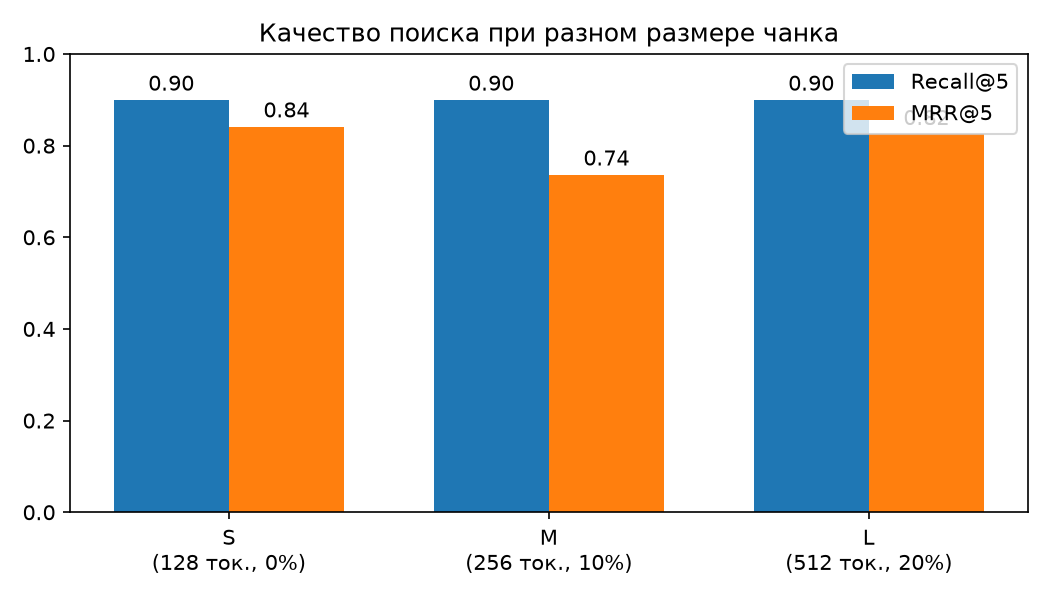
\includegraphics[width=0.78\textwidth]{part2_retrieval.png}
    \refstepcounter{figure}
    \caption*{Recall@5 и MRR@5 для конфигураций S, M и L}
    \label{fig:retrieval}
\end{figure}

Лучшая конфигурация --- \textbf{S} (MRR@5 $=0.8417$), худшая ---
\textbf{M} (MRR@5 $=0.7367$). При этом Recall@5 у всех конфигураций одинаков
(0.9000): в каждой конфигурации нашлись 18 из 20 документов, но промахи
приходятся на разные запросы. Различие проявляется не в факте попадания,
а в позиции релевантного чанка, то есть в MRR@5.

Детализация по рангам: S и L дают по 16 попаданий на первое место, однако
у L два релевантных чанка оказываются только на четвёртом месте (запросы
про еврейских игроков в Зале бейсбольной славы и про капитанов «Виннипега»),
поэтому MRR ниже. У M только 13 первых мест, два вторых, одно третье и два
пятых. Это показывает, что «оптимальный» размер чанка определяется не только
его длиной, но и выравниванием границ: короткие чанки S сохраняют локальный
сигнал, а крупные чанки L с большим перекрытием всё ещё накрывают нужный
фрагмент, тогда как промежуточный M может разрезать короткий документ неудачно.

\textbf{Разбор запроса.} Выбран запрос с опечатками
\texttt{Honda Asoct TF500 ebginner motorcycle} (документ~20, класс
\texttt{rec.motorcycles}): в S он находится на первом месте, в M не найден,
в L снова на первом. Top-5 для S и M приведены ниже (фрагменты сокращены).

\begin{lstlisting}[basicstyle=\ttfamily\footnotesize,language={}]
Query: Honda Asoct TF500 ebginner motorcycle (doc 20, rec.motorcycles)
S: rank 1; M: not found; L: rank 1.

--- top-5 for S ---
1. [OK] page=12 chars=3507-3993 (486): ... I'm going to be buying my first
   bike and I'm considering an 82 Honda Ascot FT500 with less than 5K miles ...
2. [--] page=0 chars=4138-4143 (5): t so.
3. [--] page=18 chars=2994-3567 (573): ... racing motorcycles ... flame-free ...
4. [--] page=13 chars=4360-4749 (389): ... Motorcycle Accessory Warehouse ...
5. [--] page=14 chars=3945-4506 (561): ... cafe racer ... exhaust ...

--- top-5 for M ---
1. [--] page=18 chars=2676-3780 (1104): ... riding at the edge of performance ...
2. [--] page=16 chars=932-1839 (907): ... chance of snow flurries ...
3. [--] page=19 chars=3527-4071 (544): ... not overfond of corners ...
4. [--] page=20 chars=927-1872 (945): ... Motorola Cellular APD ...
5. [--] page=18 chars=5589-5760 (171): ... subscribe euro-moto ...
\end{lstlisting}
\refstepcounter{figure}
\captionof*{figure}{Top-5 чанков для запроса про Honda Ascot: S и M}
\label{fig:case}

В S нужный фрагмент документа попал в чанк из 128 токенов, и совпадение
по редким словам \textit{Honda}, \textit{Ascot}, \textit{FT500} дало первое
место. Вероятная причина провала M --- неудачное выравнивание границ:
документ, судя по результатам, оказался на стыке двух чанков, а перекрытия
в 10\,\% (около 25 токенов) не хватило, чтобы начало документа с редкими
словами попало в один чанк. Найденные в M чанки --- это соседние сообщения
страницы с общими словами \textit{motorcycle}, \textit{riding}, \textit{bike}.
В L окно 512 токенов с перекрытием 20\,\% (около 102 токенов) снова накрыло
нужный фрагмент. Таким образом, провал M --- неудачное выравнивание границ; при выборе
размера чанка нужно учитывать и перекрытие, и фактическую длину документов.

\subsection*{Experiment Log, часть 2}

\begin{table}[H]
    \centering
    \refstepcounter{table}
    \caption*{\raggedleft Experiment Log: поиск и размер чанка}
    \label{tab:log2}
    \small
    \setlength{\tabcolsep}{6pt}
    \begin{tabular}{lrrr>{\raggedright\arraybackslash}p{0.39\textwidth}}
        \toprule
        Конфиг. & Размер & Перекр. & MRR@5 & Комментарий \\
        \midrule
        S & 128 & 0\,\%  & 0.8417 & лучший результат \\
        M & 256 & 10\,\% & 0.7367 & худший: неудачное выравнивание границ \\
        L & 512 & 20\,\% & 0.8250 & близко к S, но два попадания на 4-м месте \\
        \bottomrule
    \end{tabular}
\end{table}

\subsection{Часть 3. RAG: итеративное улучшение промпта}

\textbf{Архитектура.} Гибридный поиск объединяет плотный поиск лучшей
конфигурации части~2 и разреженный BM25 методом Reciprocal Rank Fusion (RRF,
$k_{RRF}=60$); в контекст передаются top-3 фрагмента с метками \texttt{[Doc N]}.
Генератор --- \texttt{Qwen/Qwen2.5-0.5B-Instruct}, декодирование жадное,
\texttt{max\_new\_tokens=150}. Тестовый набор: 10 вопросов с ответом в базе
(эталон --- короткая строка) и 5 вопросов без ответа про травмы игроков
(Гретцки, Лемье, Буре, Гашек, Хоу).

Вопросы задаются по-русски, но для поиска используется их английский перевод:
база знаний англоязычная, и BM25 по русской строке не находит совпадений.
Ответ генератора остаётся на русском. Отказом считается ответ с маркером
«Нет данных» (а также его английские аналоги \textit{no data},
\textit{no information}, \textit{not mentioned}).

\textbf{Промпты.} Сравнивались три инструкции:
\begin{itemize}
    \item V1 (наивный): «Ответь на вопрос, используя предоставленный текст»;
    \item V2 (строгое ограничение): «Если в тексте нет информации для ответа,
          напиши „Нет данных“. Не используй свои внутренние знания. Ответь
          строго по фактам из текста»;
    \item V3 (пошаговая проверка): выделить релевантные предложения, проверить,
          отвечают ли они напрямую на вопрос, и только затем дать краткий ответ
          или написать «Нет данных».
\end{itemize}

\textbf{Метрики.} Accuracy --- доля вопросов с ответом, где ответ содержит
эталон; Refusal Rate --- доля вопросов без ответа, на которые система
ответила «Нет данных»; Faithfulness --- доля значимых слов ответа длиннее
трёх букв, встречающихся в контексте. Дополнительно посчитаны ложные отказы
(доля отказов на вопросах, где ответ в базе есть).

\begin{table}[H]
    \centering
    \refstepcounter{table}
    \caption*{\raggedleft Сравнение промптов RAG (10 + 5 вопросов)}
    \label{tab:prompts}
    \small
    \setlength{\tabcolsep}{4pt}
    \begin{tabular}{lrrrrr}
        \toprule
        Промпт & Accuracy & Refusal Rate & Faithfulness &
        Ложные отказы & Отказы без ответа \\
        \midrule
        V1 & 0.6000 & 0.2000 & 0.4436 & 0\,\%  & 20\,\%  \\
        V2 & 0.3000 & 0.8000 & 0.5375 & 30\,\% & 80\,\%  \\
        V3 & 0.3000 & 1.0000 & 0.2167 & 60\,\% & 100\,\% \\
        \bottomrule
    \end{tabular}
\end{table}

\begin{figure}[H]
    \centering
    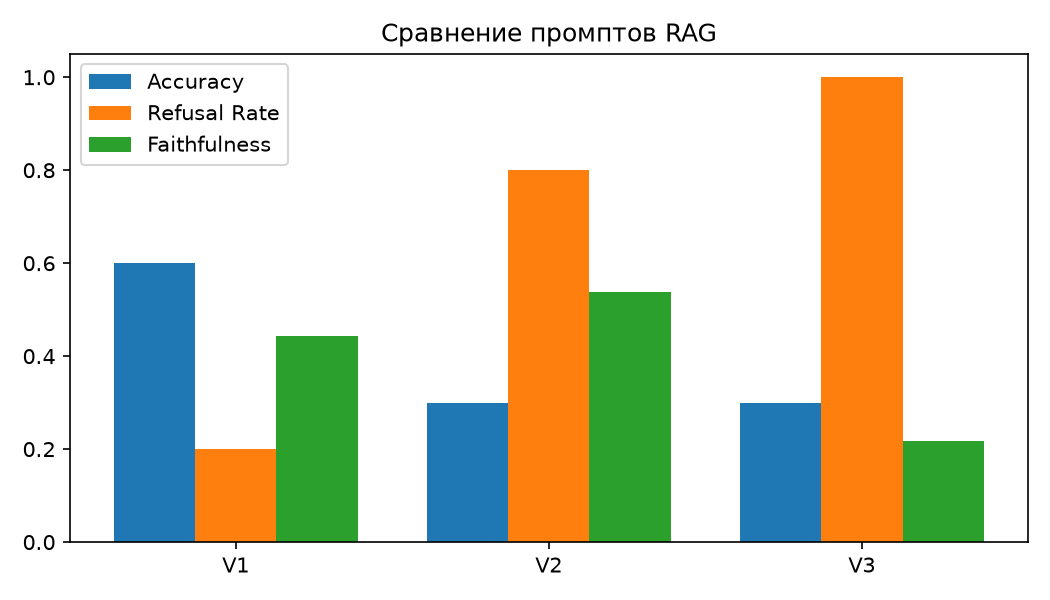
\includegraphics[width=0.78\textwidth]{part3_prompts.png}
    \refstepcounter{figure}
    \caption*{Accuracy, Refusal Rate и Faithfulness для промптов V1--V3}
    \label{fig:prompts}
\end{figure}

По компромиссному критерию
$0.4\cdot Accuracy + 0.3\cdot RefusalRate + 0.3\cdot Faithfulness$
лучший результат --- \textbf{V2}: $0.4\cdot0.3 + 0.3\cdot0.8 +
0.3\cdot0.5375 = 0.5213$; у V1 --- 0.4331, у V3 --- 0.4850.

\textbf{V1} отвечает почти всегда (ложных отказов 0\,\%), поэтому на вопросах
с ответом даёт лучшую Accuracy (0.6), но на вопросах без ответа отказывается
только в 1 случае из 5 и выдумывает факты. Например, на вопрос о травме
Гретцки V1 отвечает, что он «пропустил 3 матча», хотя в сообщениях этого нет.
\textbf{V2} снижает галлюцинации: отказывается в 4 случаях из 5, но платит
за это тремя ложными отказами (вопросы про питчера, Mercedes и смазку цепи)
и падением Accuracy до 0.3. \textbf{V3} отказывается на всех пяти вопросах
без ответа, однако ложных отказов уже 6 из 10, а Faithfulness падает до 0.2167:
короткие ответы «Нет данных» не содержат слов, подтверждённых контекстом,
и метрика штрафует их сильнее.

Характерные ответы приведены в таблице~\ref{tab:answers}.

\begin{table}[H]
    \centering
    \refstepcounter{table}
    \caption*{\raggedleft Примеры ответов V1--V3 (сокращённо)}
    \label{tab:answers}
    \footnotesize
    \begin{tabular}{>{\raggedright\arraybackslash}p{0.30\textwidth}%
                    >{\raggedright\arraybackslash}p{0.22\textwidth}%
                    >{\raggedright\arraybackslash}p{0.20\textwidth}%
                    >{\raggedright\arraybackslash}p{0.20\textwidth}}
        \toprule
        Вопрос & V1 & V2 & V3 \\
        \midrule
        Сколько секунд отводится питчеру? (эталон 20) &
        «не более 20 секунд» & Нет данных & Нет данных \\
        \addlinespace
        Сколько голов забили «Айлендерс»? (эталон 4) &
        2 & 4 & Нет данных \\
        \addlinespace
        Сколько стоит джерси Oaks? (эталон 165) &
        \$165.00 & 39 Home & \$165.00 \\
        \addlinespace
        Какую травму получил Гретцки? (ответа нет) &
        «пропустил 3 матча» & Нет данных & Нет данных \\
        \bottomrule
    \end{tabular}
\end{table}

Faithfulness в этой работе нужно трактовать осторожно: ответы генератора
русскоязычные, а контекст англоязычный, поэтому лексическое пересечение слов
занижает метрику даже для правильных ответов (например, правильный ответ
«1972» состоит из одного числового токена, а русские формулировки вокруг него
не совпадают с английским контекстом). Метрика полезна для сравнения промптов
между собой, но не как абсолютная оценка фактической точности.

\textbf{Узкое место.} Поиск нашёл документ-источник для всех 10 вопросов
с ответом (retrieval hit = 100\,\%), а классификатор части~1 даёт Accuracy 0.75;
при этом лучшая Accuracy RAG --- только 0.60. Следовательно, основное узкое
место --- не поиск и не классификатор, а генератор и формулировка инструкции:
модель теряет числа, путает соседние факты и без строгого запрета выдумывает
ответы на вопросы, которых нет в базе.

\textbf{Выбор для продакшена.} Выбран \textbf{V2}: он даёт лучший компромисс
по выбранному критерию и заметно снижает число выдуманных ответов. При этом
у него остаются ложные отказы (30\,\%), а у V3 надёжность достигается ценой
ещё большего числа ложных отказов (60\,\%). Если галлюцинация дороже отказа,
стоит выбирать V2/V3; если важнее покрытие --- V1, но только с обязательной
проверкой человеком.

\subsection*{Experiment Log, часть 3}

\begin{table}[H]
    \centering
    \refstepcounter{table}
    \caption*{\raggedleft Experiment Log: промпты RAG}
    \label{tab:log3}
    \small
    \begin{tabular}{l r l >{\raggedright\arraybackslash}p{0.40\textwidth}}
        \toprule
        Промпт & Набор & Refusal Rate & Комментарий \\
        \midrule
        V1 & 10+5 вопросов & 0.2000 & Accuracy 0.6000, много галлюцинаций \\
        V2 & 10+5 вопросов & 0.8000 & Accuracy 0.3000, лучший компромисс \\
        V3 & 10+5 вопросов & 1.0000 & Accuracy 0.3000, слишком много ложных отказов \\
        \bottomrule
    \end{tabular}
\end{table}

\section{AI Audit}

Весь код лабораторной (структура скрипта, функции \texttt{make\_pool},
\texttt{split\_chunks}, \texttt{hybrid}, \texttt{faithfulness}, сборка отчёта)
сгенерирован с помощью ИИ и проверен запуском: все три части выполнены
end-to-end, метрики взяты из реального прогона (файлы
\texttt{results/part1\_metrics.json}, \texttt{part2\_metrics.json},
\texttt{part3\_metrics.json}, логи в \texttt{logs/}).

Проверялись граничные случаи: пустые тексты (фильтр в \texttt{make\_pool}),
документы короче чанка (попадание по пересечению границ), отсутствие ответа
(Refusal Rate), совпадение границ чанков, несериализуемые типы numpy при
записи JSON. Отдельно проверено, что вопросы без ответа действительно не
содержат ответа в базе (поиск по словам \textit{injur}, \textit{knee},
\textit{wrist} и именам игроков).

Примеры ошибок ИИ и исправлений:
\begin{enumerate}
    \item первый вариант сохранения метрик через \texttt{json.dump} падал
          на \texttt{numpy.int64} в поле \texttt{count}; исправлено приведением
          к \texttt{int};
    \item выбор показательного запроса только среди лучшей и худшей
          конфигураций давал ложное «не найден», хотя запрос находился
          на первом месте; исправлено проверкой рангов и запасным выбором
          максимальной разницы;
    \item первая версия части~3 искала по русской формулировке вопроса,
          из-за чего BM25 не находил совпадений в англоязычной базе;
          исправлено добавлением английского перевода \texttt{question\_en}
          для поиска при сохранении русского вопроса в промпте;
\end{enumerate}

\section{Воспроизводимость}

Все эксперименты воспроизводятся скриптом \texttt{lr3.py}; кэш данных
лежит в \texttt{cache/}, результаты --- в \texttt{results/}, логи ---
в \texttt{logs/}. Команды запуска:

\begin{lstlisting}[language=bash]
.venv/bin/python lr3.py --part 1   # classification (CPU training, about 1.5 h)
HF_HUB_OFFLINE=1 .venv/bin/python lr3.py --part 2   # retrieval and chunks
HF_HUB_OFFLINE=1 .venv/bin/python lr3.py --part 3   # RAG and prompts
.venv/bin/python lr3.py --part report              # build the Markdown report
\end{lstlisting}

\section{Вывод}

В ходе лабораторной работы выполнены все три части варианта~16.

\begin{enumerate}
    \item \textbf{Классификация.} Дообучение \texttt{rubert-tiny2} подняло
          Accuracy с 0.3381 до 0.7535 и F1-macro с 0.2858 до 0.7510
          (прирост $+0.4155$ и $+0.4652$). Основные ошибки ---
          \texttt{rec.sport.baseball} $\to$ \texttt{rec.sport.hockey}
          (57 ошибок) и \texttt{rec.autos} $\leftrightarrow$
          \texttt{rec.motorcycles} (43 и 24 ошибки): классы тематически близки
          и делят общую лексику.
    \item \textbf{Поиск.} Recall@5 у всех конфигураций одинаков (0.9000),
          но MRR@5 максимален у S (0.8417), а минимален у M (0.7367).
          Размер чанка и перекрытие влияют не столько на факт попадания,
          сколько на позицию релевантного фрагмента; провал M, вероятно,
          объясняется неудачным выравниванием границ, а не общим «размыванием»
          сигнала.
    \item \textbf{RAG.} Гибридный поиск (BM25 + dense, RRF) находил источник
          для всех 10 вопросов с ответом. Лучший промпт --- V2: Accuracy 0.3,
          Refusal Rate 0.8, Faithfulness 0.5375, компромиссный балл 0.5213.
          V1 точнее отвечает на вопросы с ответом (0.6), но галлюцинирует
          на вопросах без ответа; V3 отказывается всегда, но даёт 60\,\%
          ложных отказов. Узкое место RAG --- генератор и инструкция, а не
          поиск.
\end{enumerate}

Итог: классификатор и поиск работают достаточно надёжно для своей части
конвейера, а качество RAG ограничено генератором. Для продакшена выбран V2
с обязательной проверкой ложных отказов; при необходимости повысить покрытие
можно вернуться к V1, но только с ручной верификацией ответов.

\appendix
\section{Сводный Experiment Log}

\begin{table}[H]
    \centering
    \refstepcounter{table}
    \caption*{\raggedleft Сводная таблица экспериментов}
    \label{tab:logall}
    \small
    \begin{tabular}{l >{\raggedright\arraybackslash}p{0.24\textwidth}%
                    >{\raggedright\arraybackslash}p{0.19\textwidth}%
                    r >{\raggedright\arraybackslash}p{0.24\textwidth}}
        \toprule
        Часть & Параметр 1 & Параметр 2 & Метрика & Результат \\
        \midrule
        Часть 1 & дообучение rubert-tiny2 & 5 эпох, lr $2\cdot10^{-5}$ &
        F1-macro & 0.7510 \\
        Часть 1 & косинус без обучения & 4 класса & F1-macro & 0.2858 \\
        Часть 2 & чанк 128 & перекрытие 0\,\% & MRR@5 & 0.8417 \\
        Часть 2 & чанк 256 & перекрытие 10\,\% & MRR@5 & 0.7367 \\
        Часть 2 & чанк 512 & перекрытие 20\,\% & MRR@5 & 0.8250 \\
        Часть 3 & промпт V1 & 10+5 вопросов & Refusal Rate & 0.2000 \\
        Часть 3 & промпт V2 & 10+5 вопросов & Refusal Rate & 0.8000 \\
        Часть 3 & промпт V3 & 10+5 вопросов & Refusal Rate & 1.0000 \\
        \bottomrule
    \end{tabular}
\end{table}

\end{document}
